%----------------------------------------------------------------------------------------
%	PACKAGES AND DOCUMENT CONFIGURATIONS
%----------------------------------------------------------------------------------------

\documentclass{article}

\usepackage{graphicx} % Required for the inclusion of images
\usepackage{natbib} % Required to change bibliography style to APA
\usepackage{amsmath} % Required for some math elements 
\usepackage{placeins}
\usepackage[font=small,labelsep=space]{caption}
\captionsetup{%
  figurename=Fig.,
  tablename=Table
}
\setcitestyle{square}
\setlength\parindent{0pt} % Removes all indentation from paragraphs

\renewcommand{\eqref}[1]{\textup{{\normalfont(\ref{#1}}\normalfont)}}

\renewcommand{\labelenumi}{\alph{enumi}.} % Make numbering in the enumerate environment by letter rather than number (e.g. section 6)

%\usepackage{times} % Uncomment to use the Times New Roman font

\textheight=8.5in
\topmargin=-0.5in

%----------------------------------------------------------------------------------------
%	DOCUMENT INFORMATION
%----------------------------------------------------------------------------------------

\title{Homework 6} % Title

\author{Kenneth \textsc{Chaney}} % Author name

\date{\today} % Date for the report

\begin{document}

\maketitle % Insert the title, author and date

\begin{center}
\begin{tabular}{l r}
Instructor: & Professor Dandekar \\ % Instructor/supervisor
Class: & ECET-512
\end{tabular}
\end{center}

% If you wish to include an abstract, uncomment the lines below
%\begin{abstract}

%\end{abstract}

\pagebreak
%----------------------------------------------------------------------------------------
%	SECTION 1
%----------------------------------------------------------------------------------------

\section{Part A}\label{partA}

To generate results for this section run the demoA.m file. The animation generated shows the mobile user traveling
across a cell while the antenna array tracks the user. There are several accompanying plots shown in figure
\ref{parta}--this is just one frame from the demoA.avi movie in the doc folder.\\


\begin{figure}[h]
\centerline{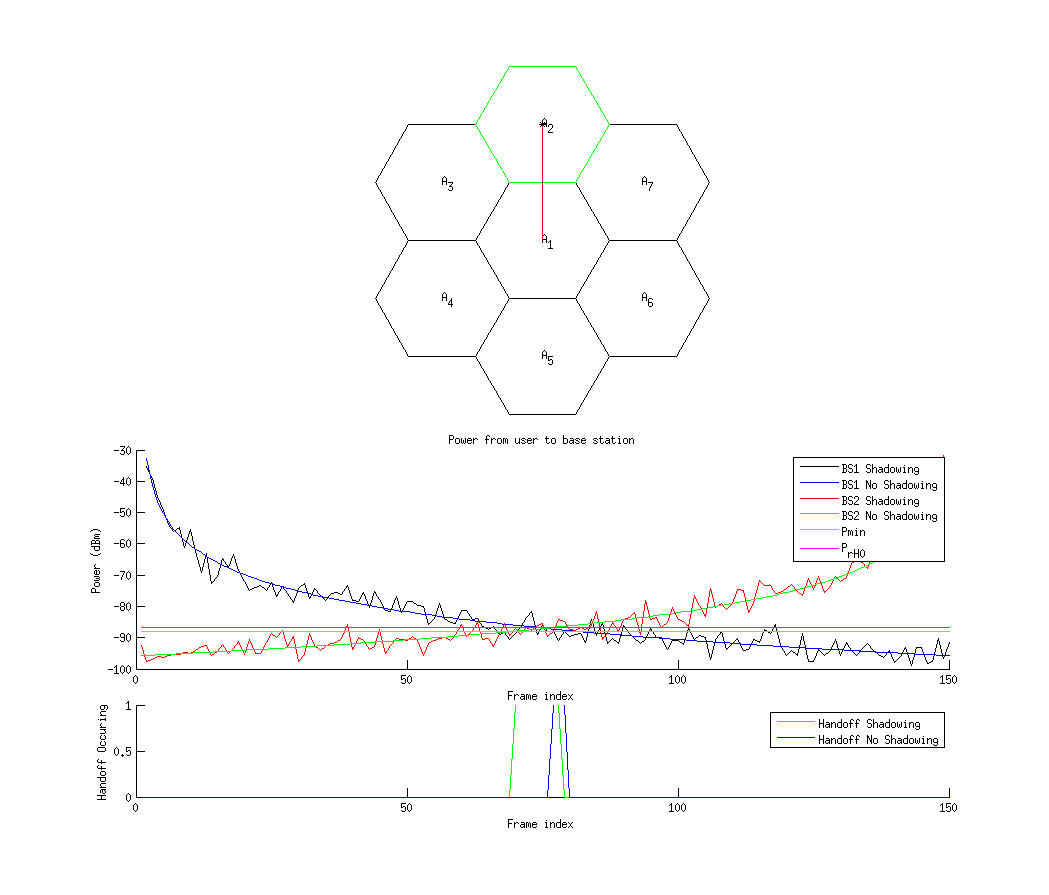
\includegraphics[width=5in]{doc/partA.png}}
\caption{Single frame of user moving through the cell while the antenna array tracks movement.}
\label{parta}
\end{figure}

\clearpage

\section{Part B}\label{partB}

To generate results for this section run the demoB.m file. A similar animation to Part A will show up--however the
distance between antennas will be varying instead of the user's location. This allows for observations as to when the
DOA estimate starts to break down because of aliasing. \\


\begin{figure}[h]
\centerline{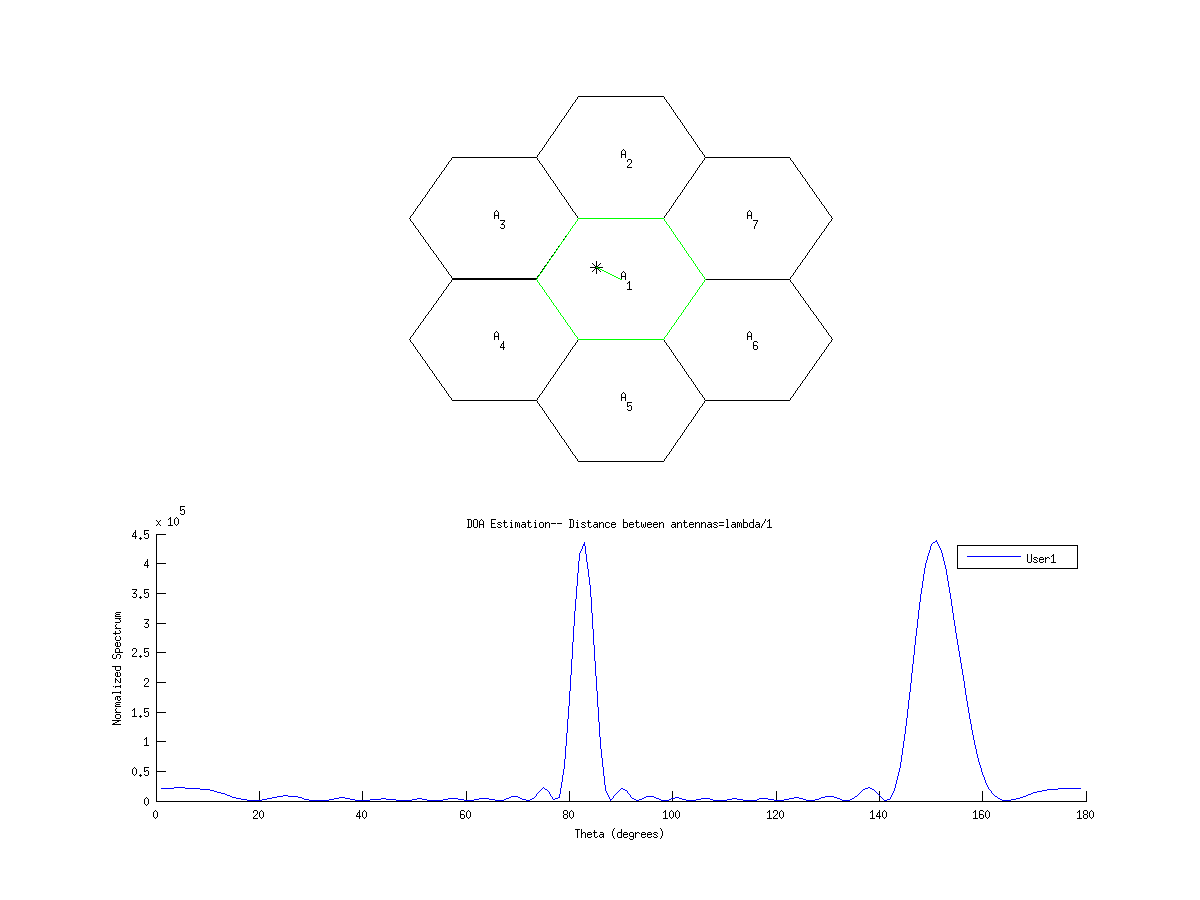
\includegraphics[width=5in]{doc/partB1.png}}
\caption{Single stationary user with antennas at lambda/1 apart.}
\label{partb1}
\end{figure}

\begin{figure}[h]
\centerline{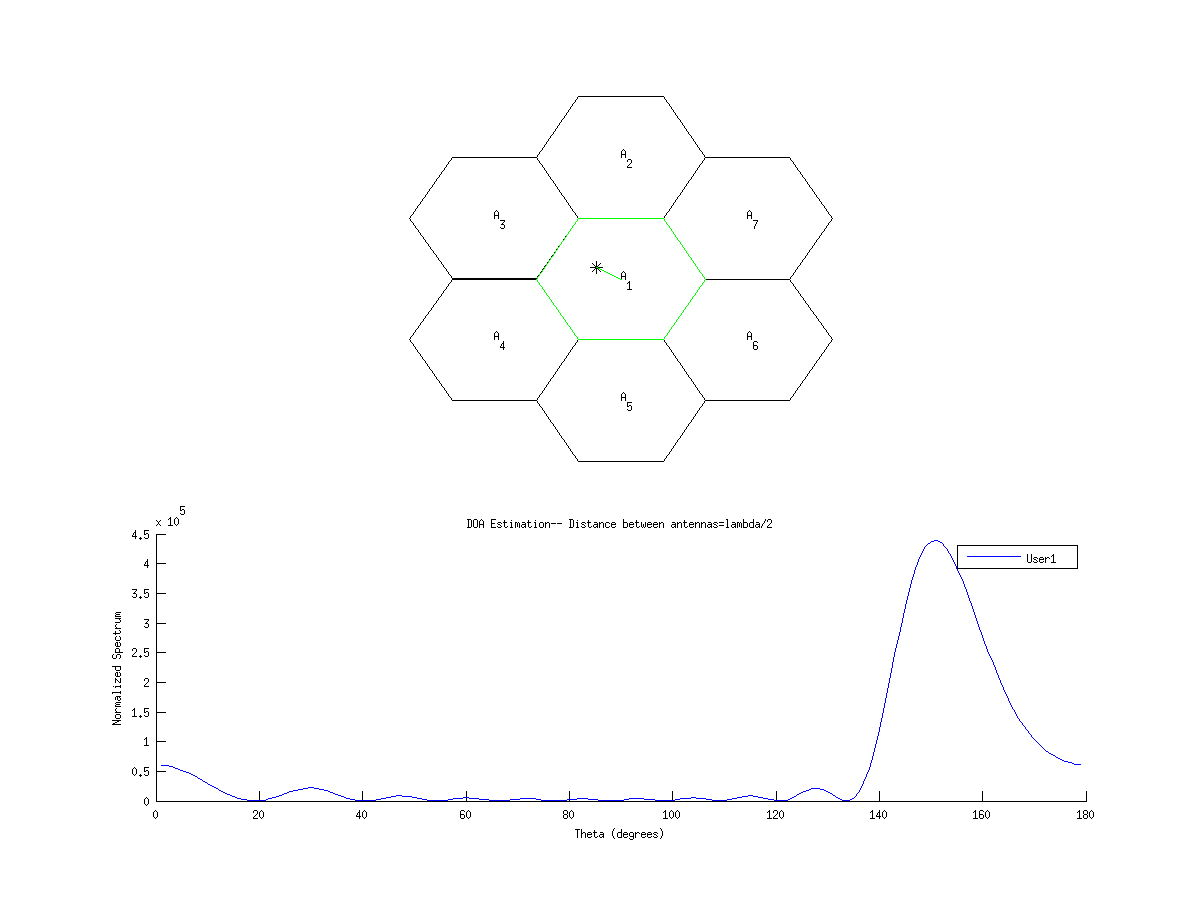
\includegraphics[width=5in]{doc/partB2.png}}
\caption{Single stationary user with antennas at lambda/2 apart.}
\label{partb2}
\end{figure}


\begin{figure}[h]
\centerline{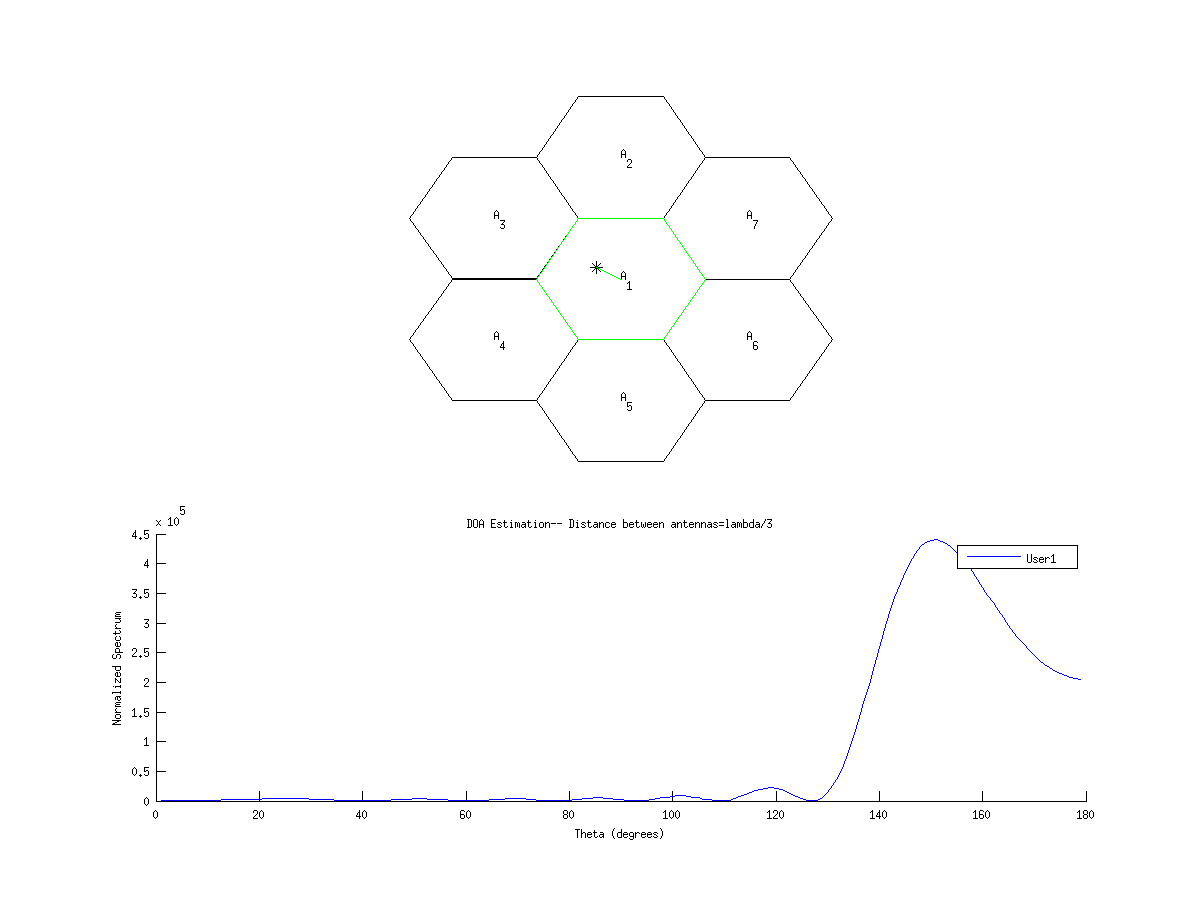
\includegraphics[width=5in]{doc/partB3.png}}
\caption{Single stationary user with antennas at lambda/3 apart.}
\label{partb3}
\end{figure}

\begin{figure}[h]
\centerline{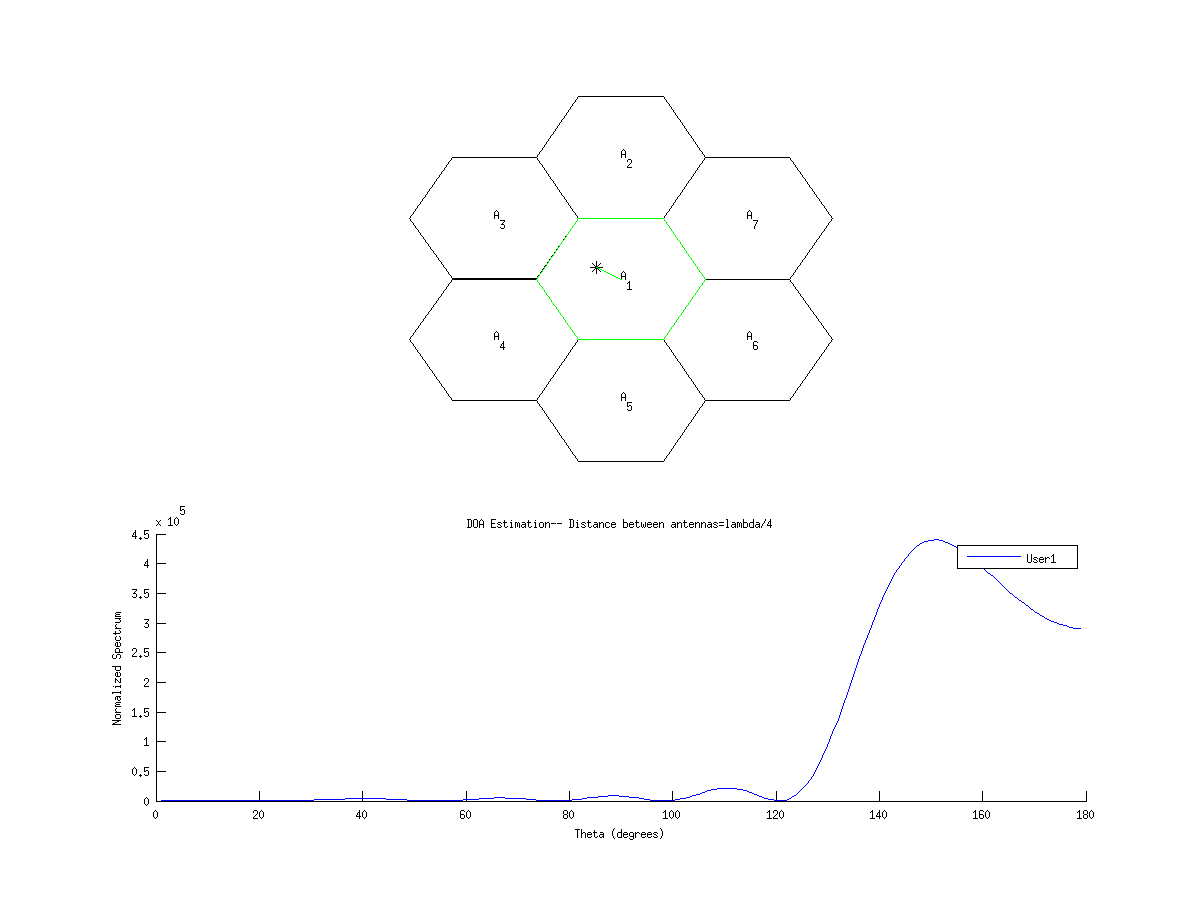
\includegraphics[width=5in]{doc/partB4.png}}
\caption{Single stationary user with antennas at lambda/4 apart.}
\label{partb4}
\end{figure}

\begin{figure}[h]
\centerline{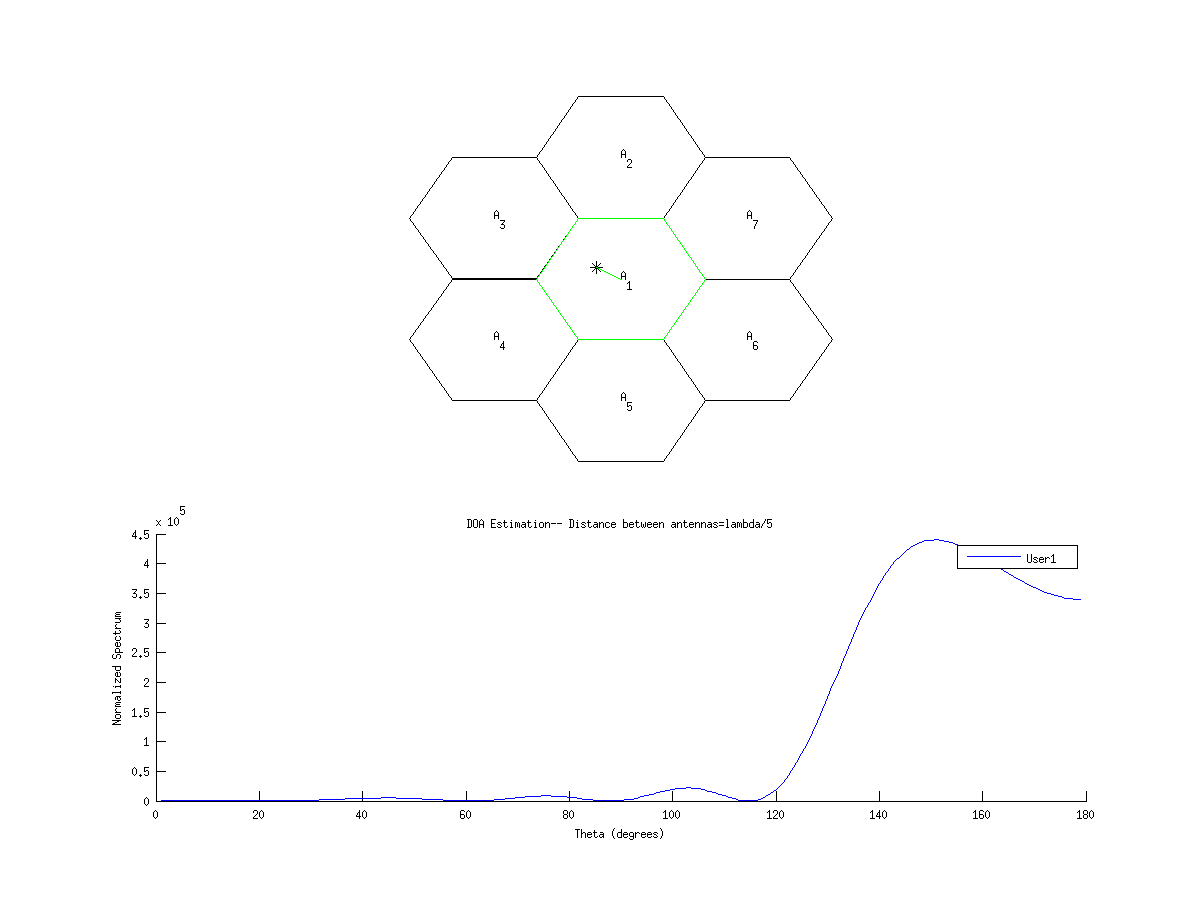
\includegraphics[width=5in]{doc/partB5.png}}
\caption{Single stationary user with antennas at lambda/5 apart.}
\label{partb5}
\end{figure}

\begin{figure}[h]
\centerline{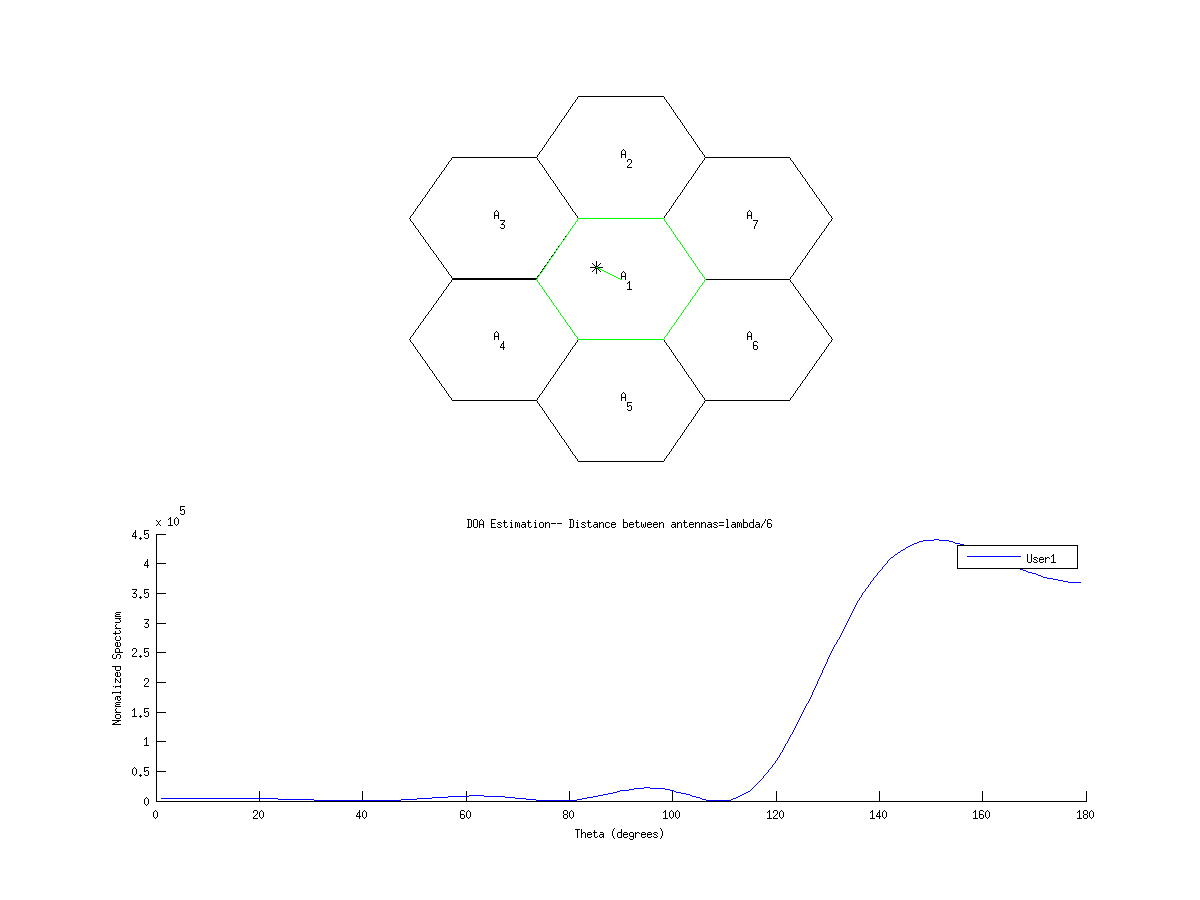
\includegraphics[width=5in]{doc/partB6.png}}
\caption{Single stationary user with antennas at lambda/6 apart.}
\label{partb6}
\end{figure}

\begin{figure}[h]
\centerline{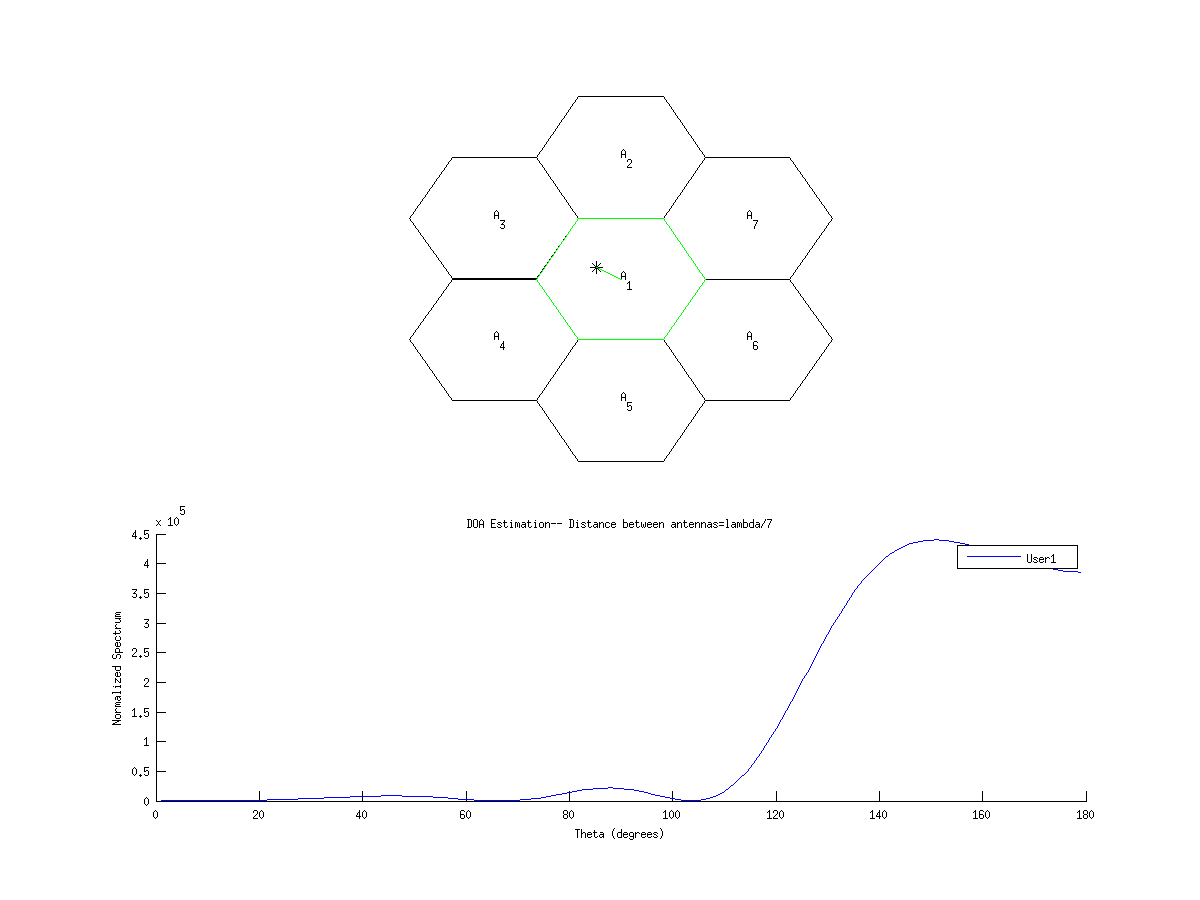
\includegraphics[width=5in]{doc/partB7.png}}
\caption{Single stationary user with antennas at lambda/7 apart.}
\label{partb7}
\end{figure}

\begin{figure}[h]
\centerline{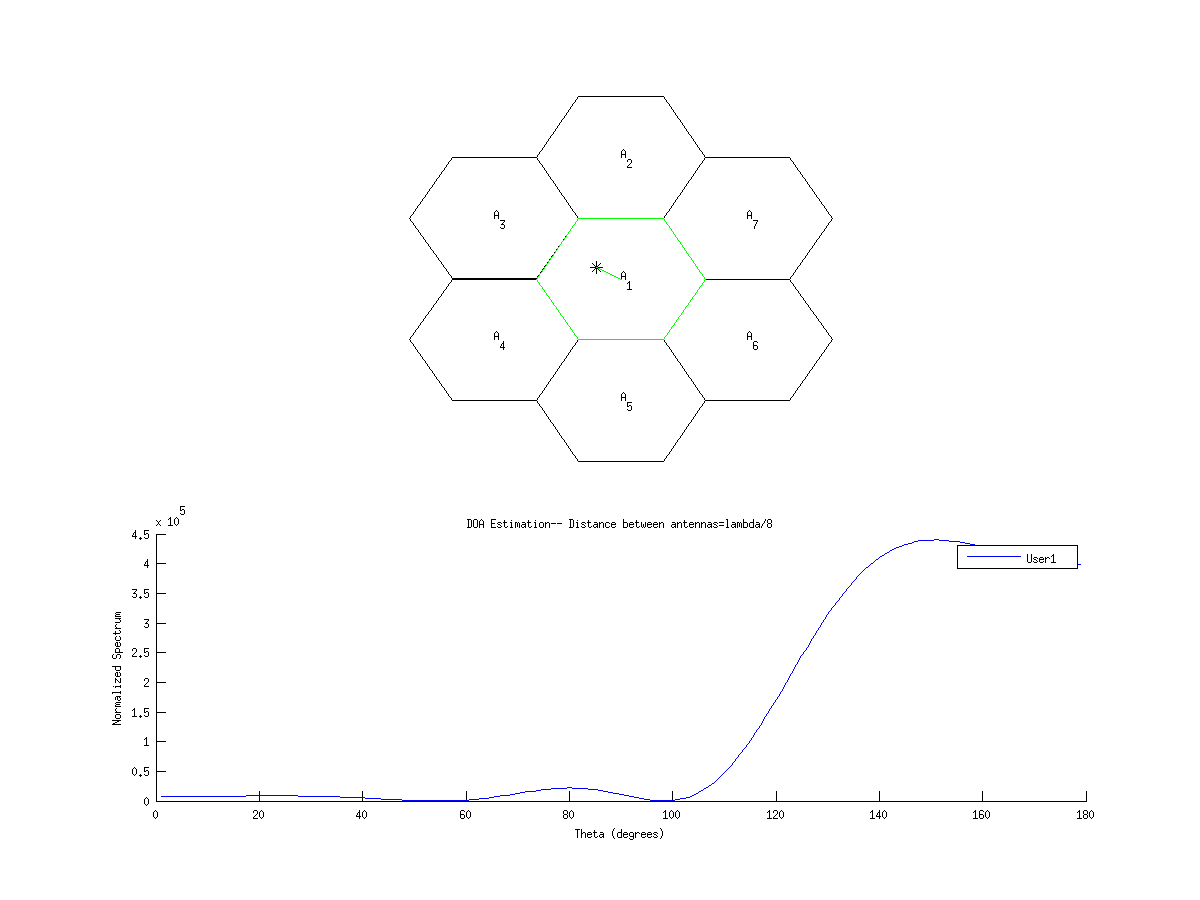
\includegraphics[width=5in]{doc/partB8.png}}
\caption{Single stationary user with antennas at lambda/8 apart.}
\label{partb8}
\end{figure}

\begin{figure}[h]
\centerline{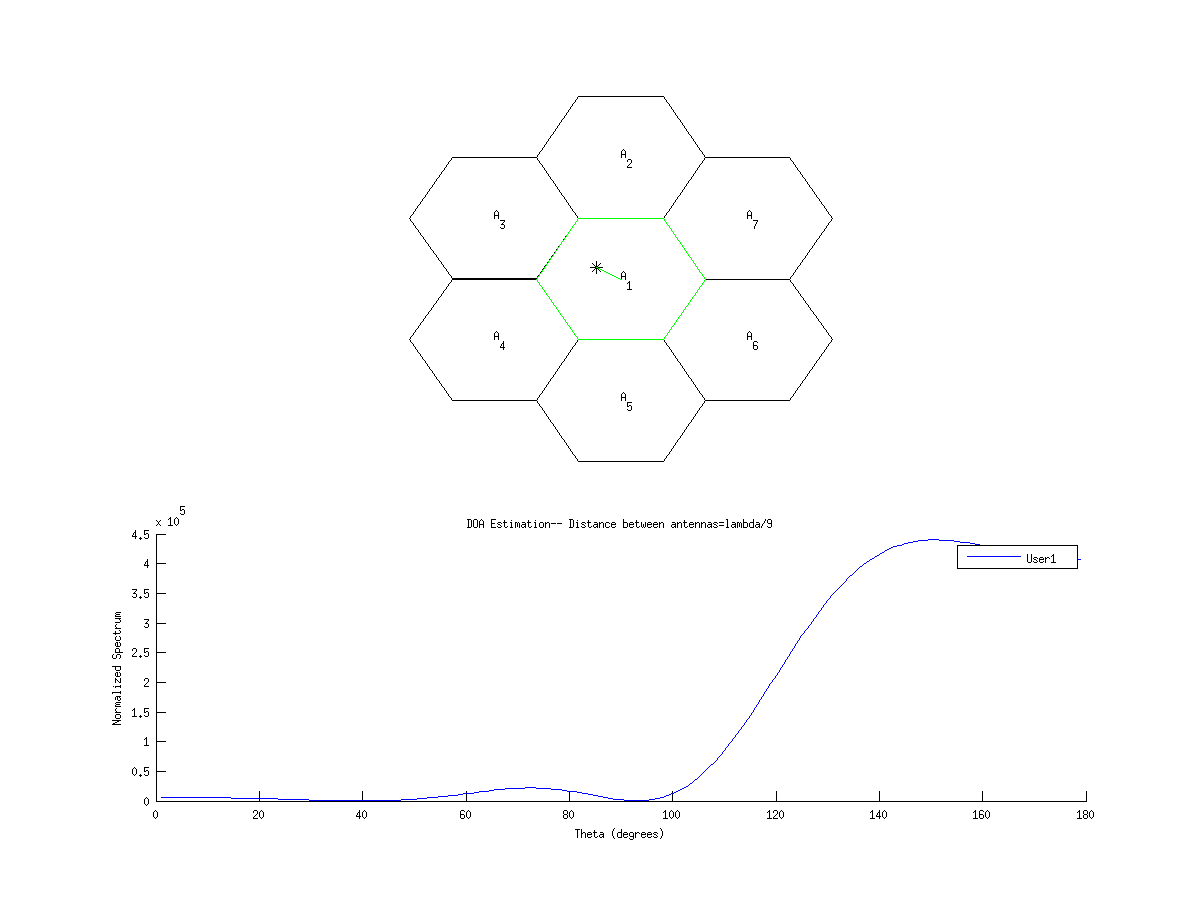
\includegraphics[width=5in]{doc/partB9.png}}
\caption{Single stationary user with antennas at lambda/9 apart.}
\label{partb9}
\end{figure}

\begin{figure}[h]
\centerline{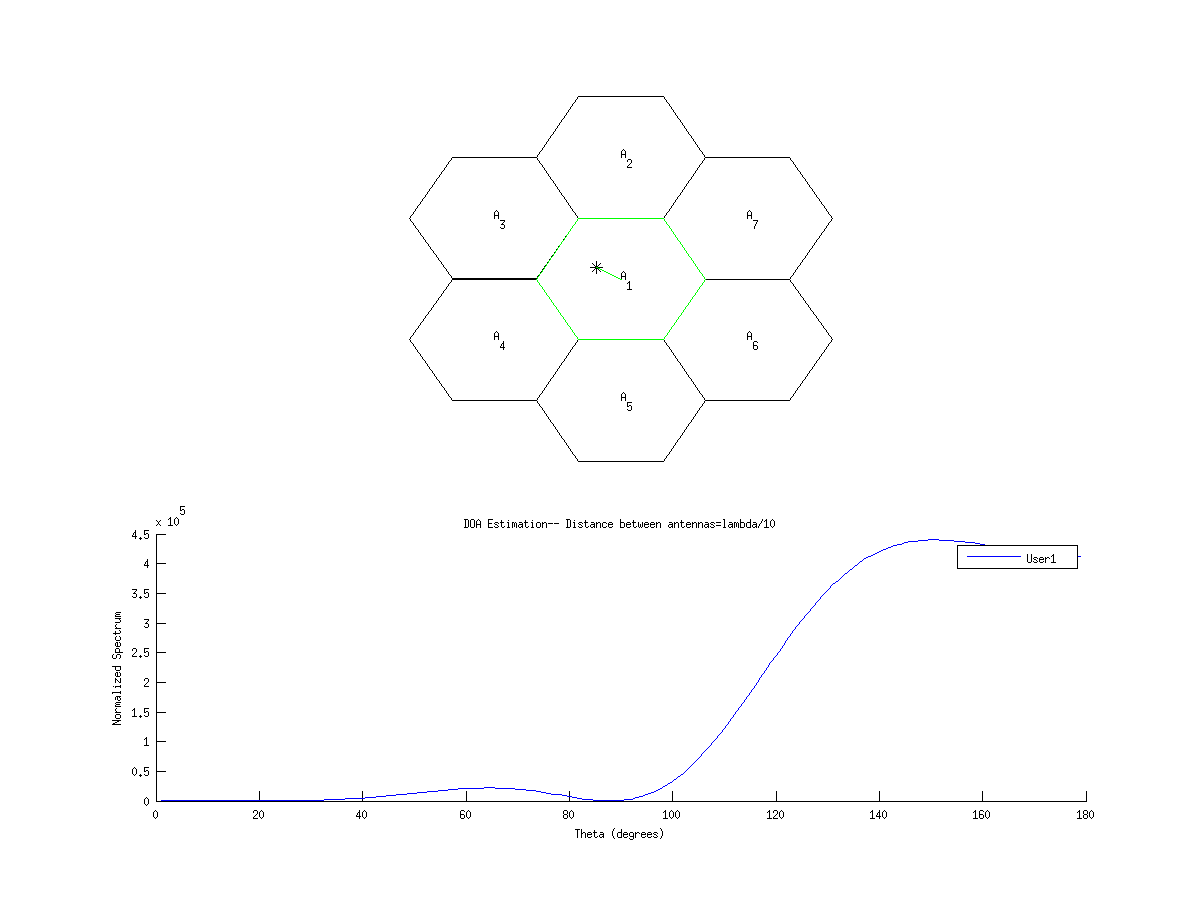
\includegraphics[width=5in]{doc/partB10.png}}
\caption{Single stationary user with antennas at lambda/10 apart.}
\label{partb10}
\end{figure}

\clearpage

\section{Part C}\label{partC}

To generate results for this section run the demoB.m file. A similar animation to Part A will show up--a sample figure is shown in figure \ref{partc}. \\


\begin{figure}[h]
\centerline{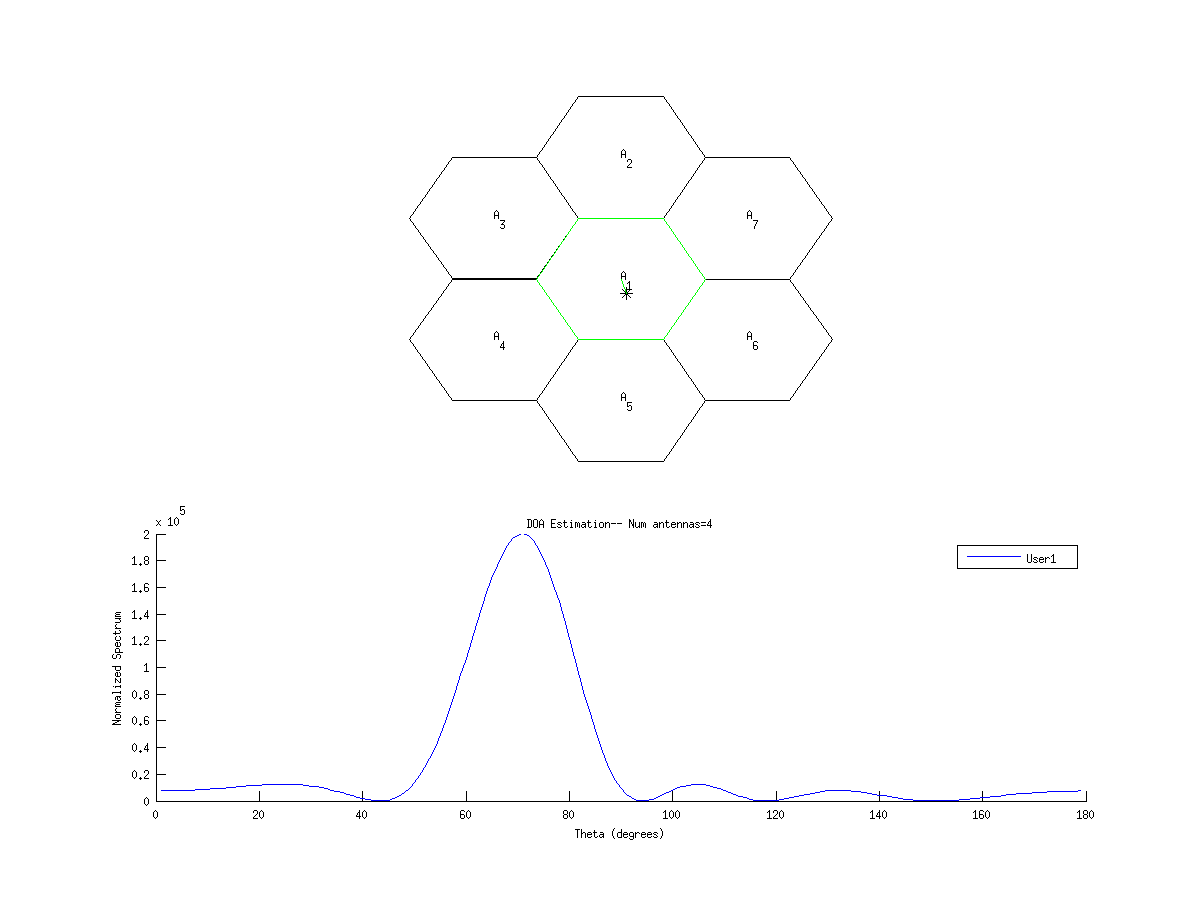
\includegraphics[width=5in]{doc/partC4.png}}
\caption{Single stationary user with 4 antennas lambda/2 distance apart.}
\label{partb1}
\end{figure}

\begin{figure}[h]
\centerline{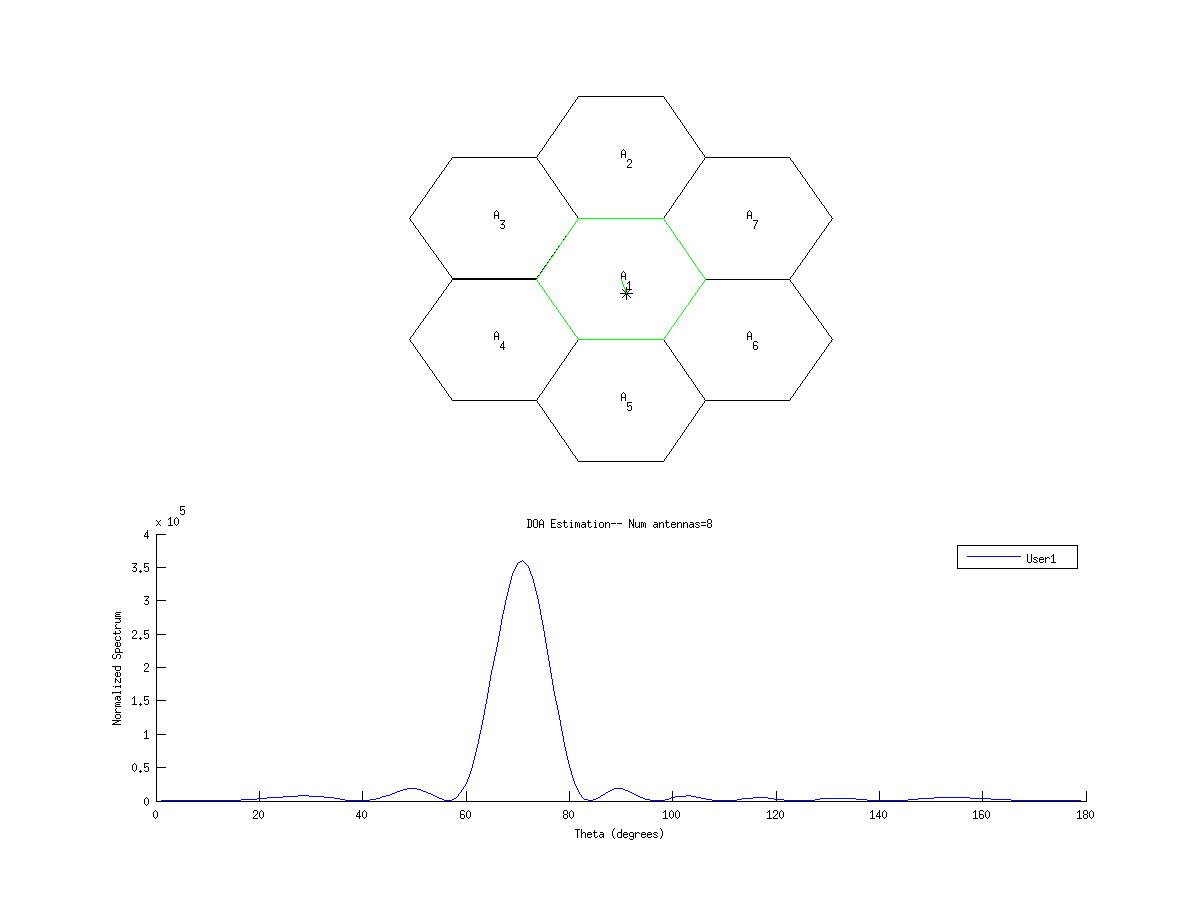
\includegraphics[width=5in]{doc/partC8.png}}
\caption{Single stationary user with 8 antennas lambda/2 distance apart.}
\label{partb1}
\end{figure}


\begin{figure}[h]
\centerline{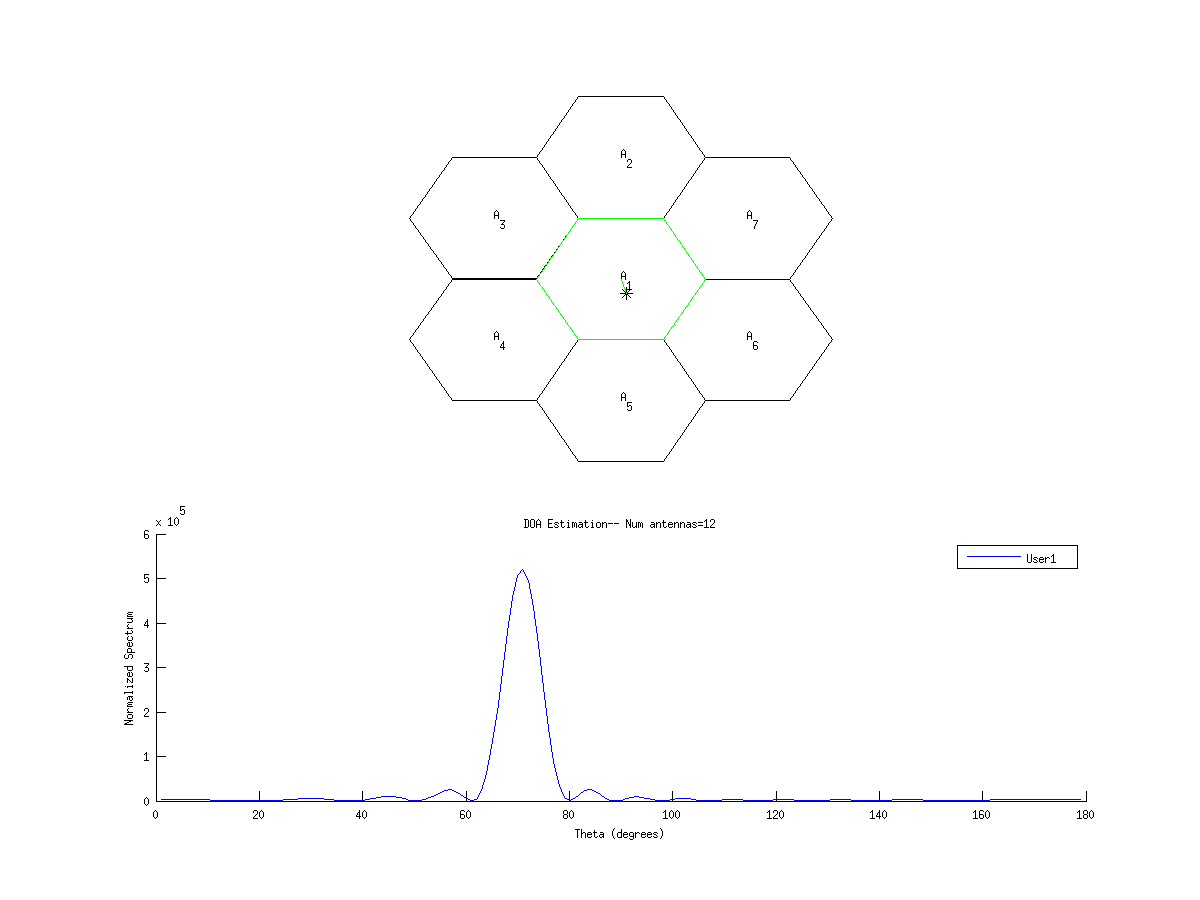
\includegraphics[width=5in]{doc/partC12.png}}
\caption{Single stationary user with 12 antennas lambda/2 distance apart.}
\label{partb1}
\end{figure}

\begin{figure}[h]
\centerline{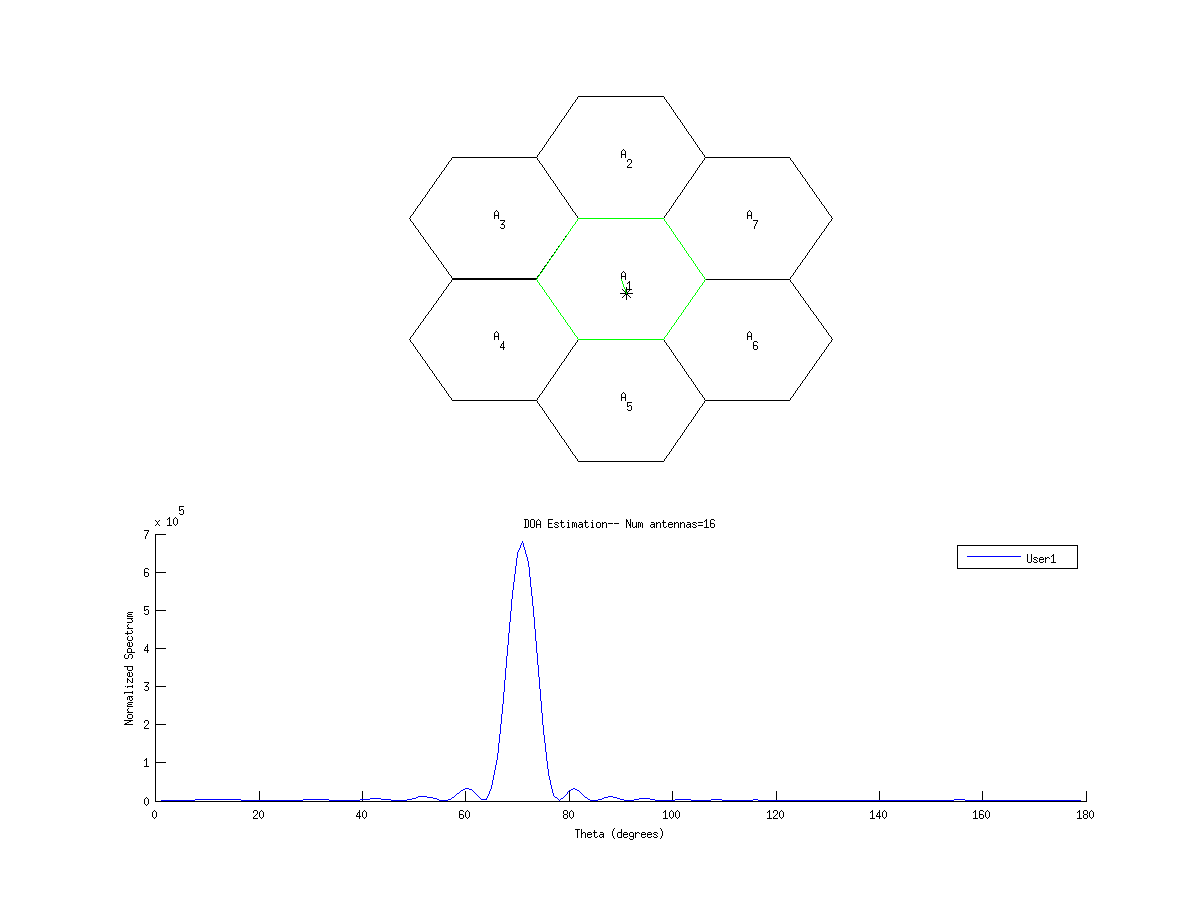
\includegraphics[width=5in]{doc/partC16.png}}
\caption{Single stationary user with 16 antennas lambda/2 distance apart.}
\label{partb1}
\end{figure}


\clearpage

\section{Part D}\label{partD}

In Part A, it was shown that the user was traveling across a portion of the environment and the antennas were able to track this movement. The tracking is very easy to see as it is shown along the bottom. While the user is crossing the axis that the antennas are on the 180 degree phase difference can be seen (i.e. this method can't determine the difference between 0 degrees and 180 degrees). However this method still provides an excellent means for tracking a singular user throughout their path.\\

In Part B, the effects of spreading out antennas was shown. As the distances got further apart the peak started to narrow giving a more accurate representation of where the user is. However once it hits \( \lambda \) distance apart aliasing is introduced into the system. \\

In Part C, there are more and more antennas added with each step. As is intuitive, the more antennas there are the better resolution you can get trying to determine where the user is. This will however never produce a perfect response at the DOA no matter how many antennas are put up.



\end{document}
